\section{Social Network}\label{sec:fa_social_network}

The current design for the escolinhas.pt social network is dynamic in nature, and extracted from the relationships formed through the connections between users and their roles with schools, groups, and even another roles, as depicted in Fig.~\ref{fig:social_network_current}. This allows the construction of a network where all the connections can be inferred dynamically and where an user can be identified another through their connections: friends, classmates, parent--child, teacher--student, and so on.

\begin{figure}[H]
  \centering
  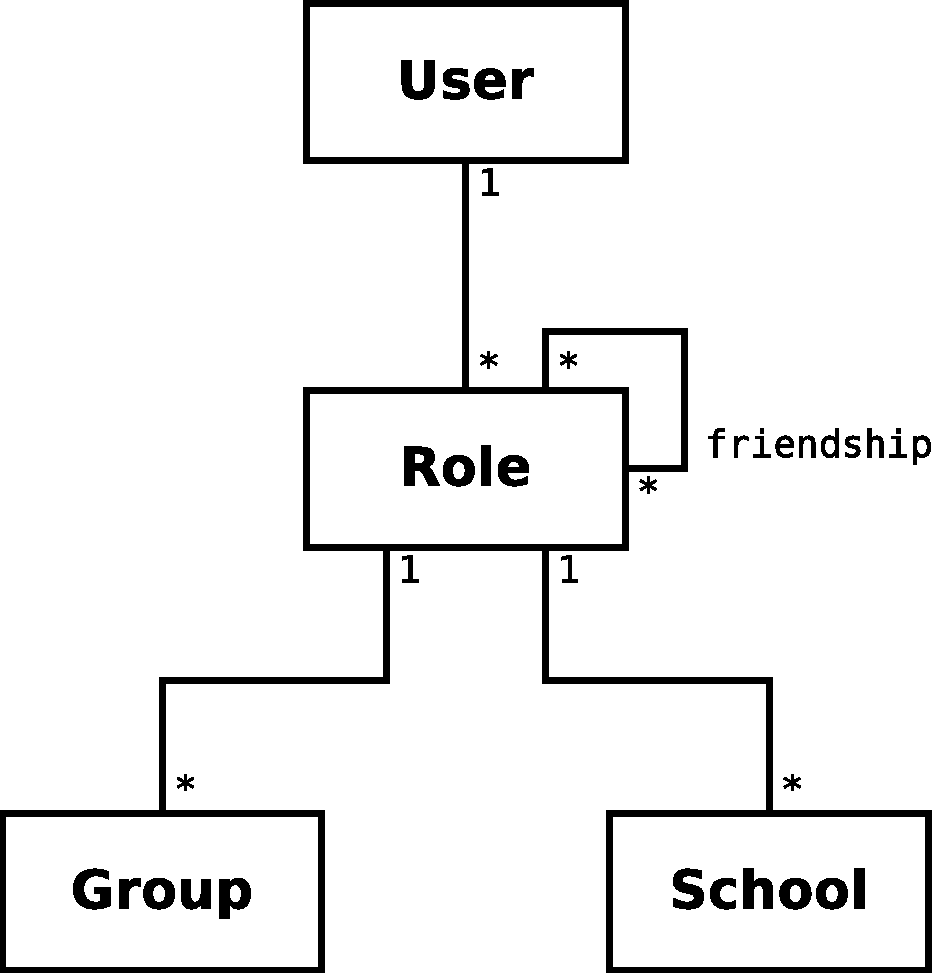
\includegraphics[width=65mm]{social_network_current.pdf}
  \caption{Current User Network Model}
  \label{fig:social_network_current}
\end{figure}

\subsection{Variability Requirements}\label{sec:fa_social_network_variability_requirements}

This model, however useful, offers a very small degree of variability. Due to the closed nature of the platform, there is a need to provide mechanisms able to fine-tune these connections in order to cater to each school specific needs. These mechanisms need to be available at the system administrator level, in order to easily manipulate these links without the need to pollute the application's codebase with hard-coded rules and without the need for redeployement.

\subsection{Candidate Patterns}\label{sec:fa_social_network_candidate_patterns}

Ideally, the user network would be described with a simple, self-referencing model, as shown in figure~\ref{fig:ideal_social_network_users}. This would allow the creation of static relationships between any two users that could be edited as needed. This would work great if all that was needed was to create realtionships between users. However, it is often necessary to create connections between users and other entities in the system, such as groups and schools. Thus, this simple model needs to be abstracted in order to connect any two entities present in the system, whichever they may be, as shown in Fig.~\ref{fig:ideal_social_network_things}.

\begin{figure}[H]
  \centering
  \subfloat[Users Network]{\label{fig:ideal_social_network_users}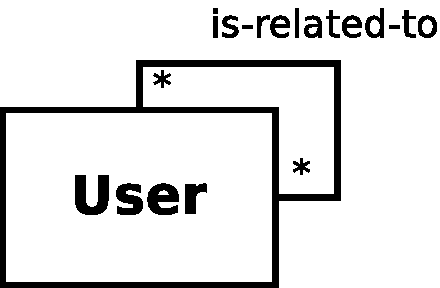
\includegraphics[width=25mm]{ideal_social_network_users}}
  \hspace{20mm}
  \subfloat[Entities Network]{\label{fig:ideal_social_network_things}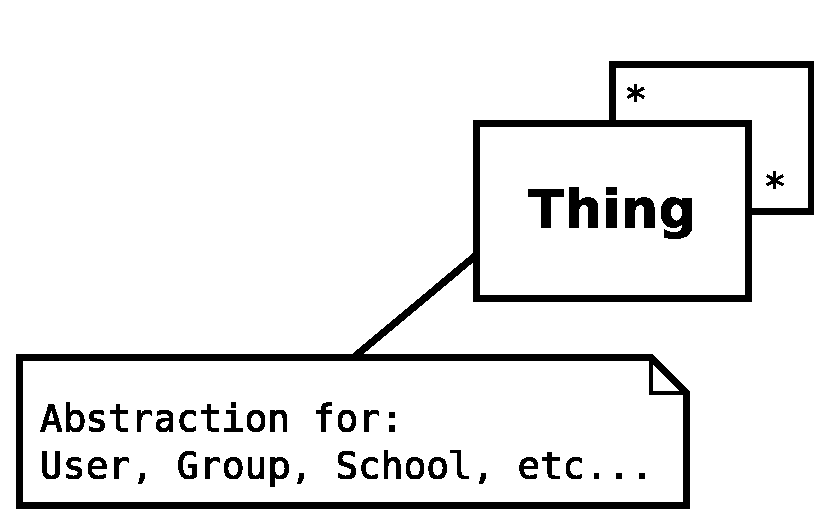
\includegraphics[width=55mm]{ideal_social_network_things}}
  \caption{Simplified Network Models}
  \label{fig:simplified_network_models}
\end{figure}

\subsection{Chosen Patterns \& Rationale}\label{sec:fa_social_network_chosen_patterns_rationale}

Despite solving the majority of the problem, the solutions described in \ref{sec:fa_social_network_candidate_patterns} are less than ideal, as they do not allow the identification of an user before another, because only a direct connection between two different entities is contemplated. As such, for this particular problem, it is necessary to be able to connect any two entities in the system, with an optional third entity to serve as hint as to how the original entities are connected. This problem can be solved by using the \textsc{Accountability} pattern (see \ref{sec:relationships_between_entities}) by Martin Fowler \cite{fowler_accountability}: it allows a bi-directional relationship between two entities (also known as \emph{parties}) while maintaining an AccountabilityType which can be used to store aditional data about the connection. As such, this AccountabilityType can be used to store an optional third party, responsible for identifying how the two other parties are connected --- effectivelly granting means to identify an user before an other, which is part of the original problem formulation (\ref{sec:fa_social_network}).

\subsection{Implementation}\label{sec:fa_social_network_implementation}

A variant of the \textsc{Accountability} design pattern was chosen (shown in Fig.~\ref{fig:social_network_conceptual}). This implementation follows the original description of the pattern by using all the usual entities present in the original \textsc{Accountability} pattern \cite{fowler_accountability} --- however, it denormalizes the AccountabilityType entity \emph{into} the Accountabilities themselves, by placing the AccountabilityType attributes (\verb!type!, \verb!through!, \verb!school_year!, \verb!active!) in the Accountability. Despite creating some data redundancy, this option provides a more performant implementation: as the Accountabilities table is to be constantly accessed, the decision to have the AccountabilityTypes in a separate table would lead to expensive \verb!JOIN! operations. This, in turn, would lead to a less than desirable performance and complexity.

\begin{figure}[H]
  \centering
  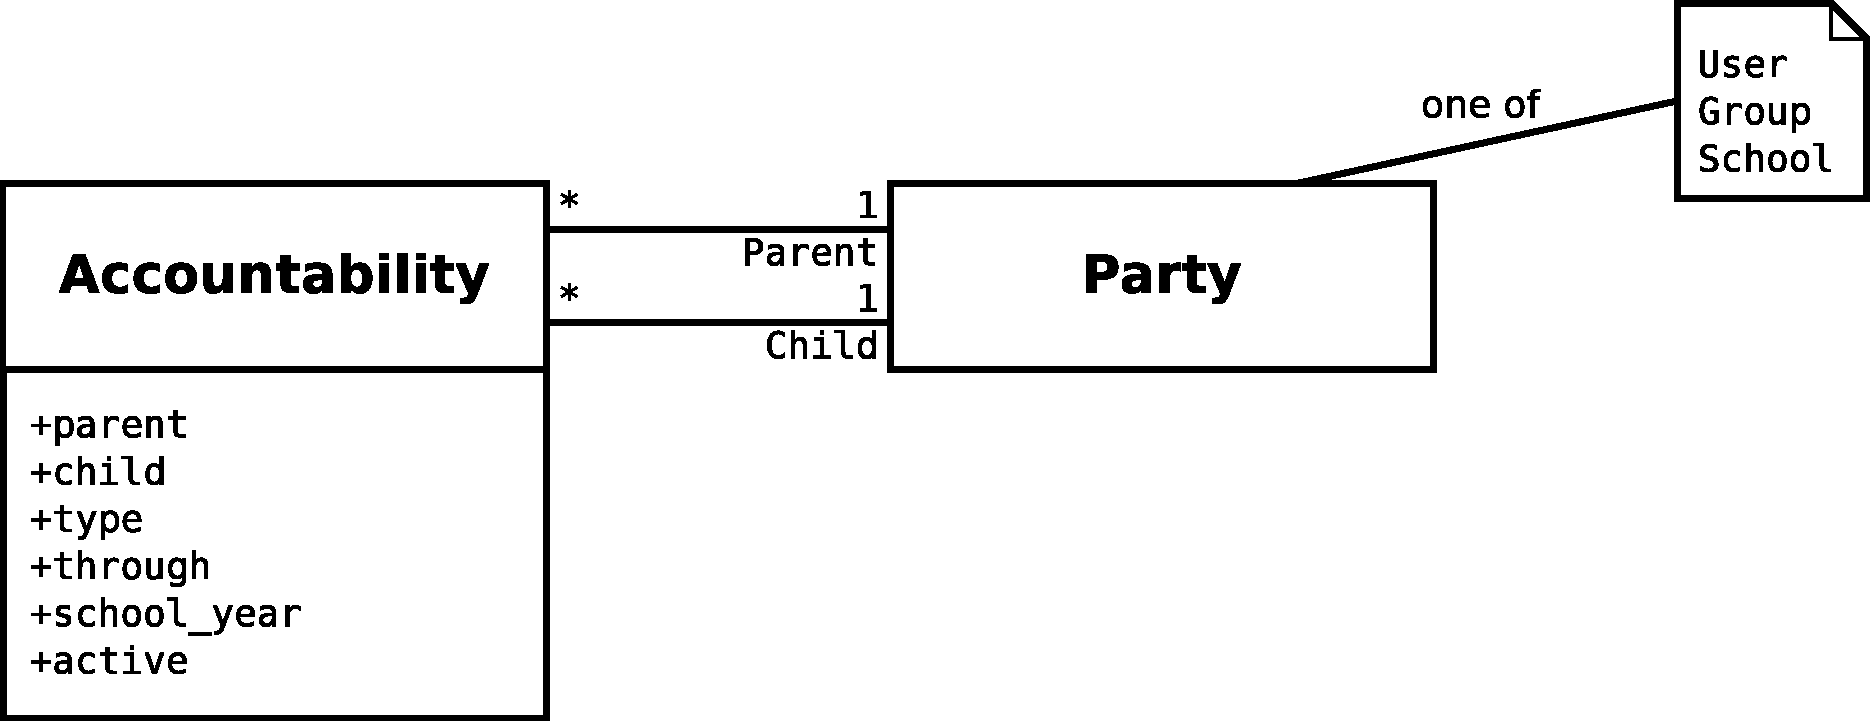
\includegraphics[width=115mm]{social_network_conceptual}
  \caption{Accountability Implementation for User Network}
  \label{fig:social_network_conceptual}
\end{figure}

The following AccountabilityTypes were created:

\begin{itemize}
  \item \textbf{group\_professor:} establishes a connection between a \emph{Group} and a \emph{Professor}, meaning that the user is one of the teacher of \emph{Group}
  \item \textbf{professor:} establishes a connection between two \emph{Users} --- a \emph{Professor} and a \emph{Student} --- creating a teacher-student relationship between them through whichever \emph{Group} they are related to
  \item \textbf{group\_student:} establishes a connection between a \emph{Group} and a \emph{Student}, meaning that the user is part of the \emph{Group} and taught by the \textbf{group\_professors} associated with the aforementioned \emph{Group}
  \item \textbf{school\_professor:} establishes a connection between a \emph{School} and a \emph{Professor}
  \item \textbf{school\_student:} establishes a connection between a \emph{School} and a \emph{Student}
  \item \textbf{parent:} establishes a parenthood relationship between two users
  \item \textbf{school\_coordinator:} dictates an \emph{User} is a coordinator (also known as an administrator) of a certain \emph{School}
  \item \textbf{colleague:} establishes a connection between two \emph{Users} --- either a \emph{Coordinator} or a \emph{Professor} --- through a \emph{School} they both work in
  \item \textbf{student:} establishes a relationship between a \emph{Coordinator} and a \emph{Student} through a \emph{School}
  \item \textbf{school\_parent:} establishes a relationship between a \emph{Coordinator} and a \emph{Parent} through a \emph{School}
  \item \textbf{friend:} establishes a connection between any two \emph{Users} of the system --- whichever their roles may be --- to indicate a friendship relation exists between them
\end{itemize}

% generated with http://truben.no/latex/table/
%\begin{table}
% \begin{tabular}{|l|l|l|l|l|}
%  \hline
%   group\_professor  & Group                 & Professor             & -      & - \\ 
%   professor         & Professor             & Student               & Group  & - \\ 
%   group_student     & Group                 & Student               & -      & - \\ 
%   school\_professor & School                & Professor             & -      & - \\ 
%   school\_student   & School                & Student               & -      & - \\ 
%   parent            & Parent                & Student               & -      & - \\ 
%   school_cordinator & School                & Coordinator           & -      & - \\ 
%   colleague         & Coordinator/Professor & Coordinator/Professor & School & - \\ 
%   student           & Coordinator           & Student               & School & - \\ 
%   school\_parent    & Coordinator           & Parent                & School & - \\ 
%   friend            & User                  & User                  & -      & - \\
%  \hline
% \end{tabular}
%\end{table}

The aforementioned AccountabilityTypes are representative of every type of interpersonal relationship existent in the escolinhas.pt platform. At first sight, some of the AccountabilityTypes created may seem redundant, such as student and school\_parent: they exist because the school coordinator needs to be able to contact everyone who is part of the school. One could argue these connections could easily be inferred through the relations between the coordinator and his or her school, and the relations existent between the school and its students, and finally use the existent parenthood relationships. However, as described in \ref{sec:fa_social_network_variability_requirements}, one of the major design flaws (regarding variability), was the completely dynamic nature of the contacts network. Thus, the choice to implement apparently redundant AccountabilityTypes tied itself with the necessity to have full controll over the existent social relationships.

\subsection{Impact Analysis}\label{sec:fa_social_network_impact_analysis}

The usage of this design pattern not only solved some of the existing variability and performance problems, but introduced a new possibility: the ability to create relationships between any two entities in the system. This leads to a very flexible network, capable of being modified at the M0 (data) level (see \ref{sec:aom_architecture}), which is a pre-requisite for end-user level variability.

A secondary objective pertaining to the application of this pattern was to improve the performance related to contact list creation and the identification of these contacts before the user. This task is currently extremely expensive, with an edge case of 5724 queries needed to fetch and identify 715 contacts. A user with only 18 contacts generates 154 queries. This means that an average of 8 queries are performed for each one of the contacts, meaning the cost of this operation is linear ($O(n)$) in nature. The implementation of the \textsc{Accountability} pattern to maintain the relationships between users was able to reduce the cost of the abovementioned task to $O(1)$: only 11 queries are performed to fetch and identify an user's contacts, regardless of the size of the contacts list.

\textbf{NOTE: should Big O notation be used to express operation costs (i.e. number of queries performed)?}







